% 113-03(인쇄 113쪽) — 유형 066 03번의 두 정규분포곡선 A, B(A 는 왼쪽·높고 좁게, B 는 오른쪽·낮고 넓게 · 대칭축 점선 없음).
% 스캔 화질이 낮아 TikZ 로 다시 그림. 라벨은 원문에 있는 것만(A, B, x)이고 평균·표준편차의 값은 적지 않는다.
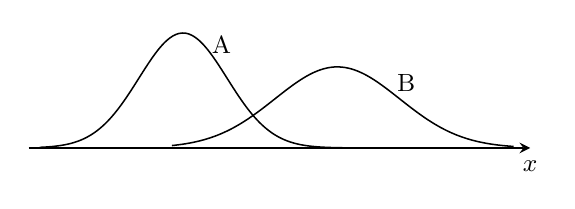
\begin{tikzpicture}[x=0.70cm, y=1.05cm, line width=0.55pt, font=\small]
  \draw[->, >=stealth, line width=0.7pt] (-4.3,0) -- (4.8,0) node[below=1pt] {$x$};
  \draw plot[domain=-4.1:1.6, samples=100, smooth] ({\x},{1.39*exp(-(\x+1.5)*(\x+1.5)/(2*0.80*0.80))});
  \draw plot[domain=-1.7:4.5, samples=100, smooth] ({\x},{0.98*exp(-(\x-1.3)*(\x-1.3)/(2*1.13*1.13))});
  \node at (-0.80,1.24) {$\mathrm{A}$};
  \node at (2.55,0.78) {$\mathrm{B}$};
\end{tikzpicture}
